\documentclass[a4paper,12pt,reqno]{amsart}
\usepackage{graphicx}
\usepackage{macros_M53}

% pour voir les solutions il faut enlever le commentaire de la ligne suivante
% \solutionstrue

\begin{document}

% ==================================
\hautdepage{

\ifsolutions{Solutions de l'examen final}\else{Examen final}\fi\par\normalfont\normalsize
4 janvier 2016\\{[ durée: 3 heures ]}\par
}
% ==================================
\ifsolutions\else
% {\fontencoding{U}\fontfamily{futs}\selectfont\char 66\relax}
\tikz[baseline=(e.base)]{\NoAutoSpacing\node(e){!};\draw[red,ultra thick,line join=round,yshift=-.15ex](90:1em)--(210:1em)--(330:1em)--cycle;}
\textbf{Documents autorisés :}\textit{Une feuille A4 recto-verso écrite à la main.}

\tsvp

\vspace{14mm}
\fi

%-----------------------------------
\begin{exo} (Question de cours et applications)
  \begin{enumerate}
    \item Démontrer la proposition du cours :

    \framebox{
      \parbox{\textwidth-3cm}{\centering\vspace{1mm}
        \emph{Soient une bijection $\phi:A\isoto B$ et une application $f:A\to C$,\\
        alors l'image de l'ensemble de niveau $\ens{L}_{k}(f\,)$ par $\phi$ est $\ens{L}_{k}(f\circ \phi^{-1}\,)$.}
      }
    }
  \end{enumerate}

  \medskip
  \emph{Pour la suite de l'exercice on se place dans $\mathbb{R}^{2}$ muni de sa base canonique.}

  \begin{enumerate}[resume]
    \item Donner l'expression analytique d'une transformation affine $\phi$ qui envoie le cercle d'équation $\{x^{2}+(y-1)^{2}=2\}$ sur l'ellipse d'équation $\{2x^{2}+y^{2}=1\}$.

    \item Existe-t-il une application définie sur $\mathbb{R}^{2}$ qui envoie l'ensemble d'équation\\ $\{2x^{2}+2xy+y^{2}+x-3y=0\}$ sur l'ensemble d'équation $\{9x^{2}+12xy+4y^{2}+1=0\}$?
  \end{enumerate}
\end{exo}

\begin{solution}
  \newcommand\circled[1]{\textcircled{\scriptsize #1}}
  \newcommand\scriptcircled[1]{\raisebox{3pt}{\scriptsize\textcircled{\raisebox{-0.3pt}{\tiny #1}}}}

  \begin{enumerate}
    \item
      $ M \in \phi(\ens{L}_{k}(f\,)) \stackrel{\scriptcircled{1}}{\ssi}
        \phi^{-1}(M) \in \ens{L}_{k}(f\,) \stackrel{\scriptcircled{2}}{\ssi}
        f(\phi^{-1}(M))=k \stackrel{\scriptcircled{3}}{\ssi}
        M \in \ens{L}_{k}(f\circ\phi^{-1}) $.
    \begin{itemize}[leftmargin=!]
      \item[\circled{1}] Car $\phi$ est une bijection.
      \item[\circled{2}+\circled{3}] Par la définition de l'ensemble de niveau $\ens{L}_{k}$.
    \end{itemize}
    \item Soit $\phi(x,y)=(\frac{x}{2},\frac{y-1}{\sqrt{2}})$, alors $\phi^{-1}(x,y)=(2x,y\sqrt{2}+1)$. Soit $f(x,y)=\frac{1}{2} x^{2}+\frac{1}{2}(y-1)^{2}$, alors $f\circ \phi^{-1}(x,y)=2x^{2}+y^{2}$, et donc l'image de l'ensemble de niveau $\ens{L}_{1}(f\,)$ par $\phi$ est $\ens{L}_{1}(f\circ \phi^{-1}\,)$.
    \item Comme $(0,0)\in\{2x^{2}+2xy+y^{2}+x-3y=0\}$ cet ensemble n'est pas vide. Comme $\{9x^{2}+12xy+4y^{2}+1=0\}=\{(3x+2y)^{2}=-1\}$ cet ensemble est vide. Aucune application ne peut envoyer un ensemble non vide dans un ensemble vide.
  \end{enumerate}
\end{solution}


%-----------------------------------
\begin{exo} (Géométrie dans $\mathbb{R}^{3}$)

  On se place dans l'espace affine euclidien $\mathbb{R}^{3}$. On considère le plan $\ens{P}$ d'équation $\{2x+y=1\}$ et la droite $\ens{D}$ d'équations $\{z=-1,\ x=y\}$.

  \begin{enumerate}

    \item Donner l'expression analytique de la projection $p$ sur le plan $\ens{P}$ suivant la direction $\ens{D}$.

    \item Donner l'expression analytique de la symétrie $s$ par rapport à $\ens{P}$ suivant la direction $\ens{D}$.

    \item Donner l'expression analytique de la projection orthogonale $\pi$ sur le plan $\ens{P}$.

    \item Calculer la distance de $A=(1,0,1)$ au plan $\ens{P}$.

    \item Donner l'expression analytique de la symétrie orthogonale $\sigma$ par rapport à $\ens{P}$.

    \item Soit $\ens{C}$ le cône standard d'équation $\{x^{2}+y^{2}-z^{2}=0\}$. Quelle est la nature de l'intersection $\ens{P} \cap \ens{C}$ ? Dessiner cette intersection.
  \end{enumerate}
\end{exo}

\begin{solution}
  \begin{enumerate}
    \item La direction de $\ens{D}$ est $\ev{D}=\{z=0,\ x=y\}=\affspan{(1,1,0)}$. Ainsi la projection recherchée d'un point de coordonnées $(x,y,z)$ est un point de coordonnées $(x+\lambda,y+\lambda,z)$ avec $2(x+\lambda)+(y+\lambda)=1$. On déduit $\lambda=\frac{1}{3}(-2x-y+1)$ et donc
    \[
      p(x,y,z)=(\frac{x-y+1}{3},\frac{-2x+2y+1}{3},z).
    \]
    \item Comme $\frac{1}{2}x+\frac{1}{2}s(x,y,z)=p(x,y,z)$ on trouve
    \[
      s(x,y,z)=(\frac{-x-2y+2}{3},\frac{-4x+y+2}{3},z).
    \]
    \item D'après l'équation de $\ens{P}$ sa direction orthogonale est $\affspan{(2,1,0)}$. Ainsi la projection recherchée d'un point de coordonnées $(x,y,z)$ est un point de coordonnées $(x+2\lambda,y+\lambda,z)$ avec $2(x+2\lambda)+(y+\lambda)=1$. On déduit $\lambda=\frac{1}{5}(-2x-y+1)$ et donc
    \[
      \pi(x,y,z)=(\frac{x-2y+2}{5},\frac{-2x+4y+1}{5},z).
    \]
    \item Nous avons $\pi(1,0,1)=(\frac{3}{5},-\frac{1}{5},1)$, d'où $d(A,\ens{P})=d(A,\pi(A))=\norm{(\frac{2}{5},\frac{1}{5},0)}=\frac{1}{\sqrt{5}}$.
    \item Comme $\frac{1}{2}x+\frac{1}{2}\sigma(x,y,z)=\pi(x,y,z)$ on trouve
    \[
      \sigma(x,y,z)=(\frac{-3x-4y+4}{5},\frac{-4x+3y+2}{5},z).
    \]
    \item Le plan $\ens{P}$ est «vertical» dans le sens que sa direction $\ev{P}=\{2x+y=0\}$ contient la direction $\affspan{(0,0,1)}$. L'intersection d'un plan «vertical» avec le cône standard est une hyperbole.\newline
    On peut voir ça aussi par les équations. Comme $\ens{P} \cap \ens{C}=\{2x+y=1, x^{2}+y^{2}=z^{2}\}$, en remplaçant $y=1-2x$ dans l'équation du cône on trouve que l'intersection $\ens{P} \cap \ens{C}$ est l'image par l'isomorphisme $(x,z)\mapsto(x,1-2x,z)$ de $\mathbb{R}^{2}$ dans $\ens{P}$ de l'hyperbole d'équation $5(x-\frac{2}{5})^{2}-z^{2}=\frac{1}{5}$.
  \end{enumerate}
\end{solution}


%-----------------------------------
\begin{exo} (Construction d'une ellipse)

  \begin{wrapfigure}{r}{59mm}
    \centering\vspace{-14mm}
    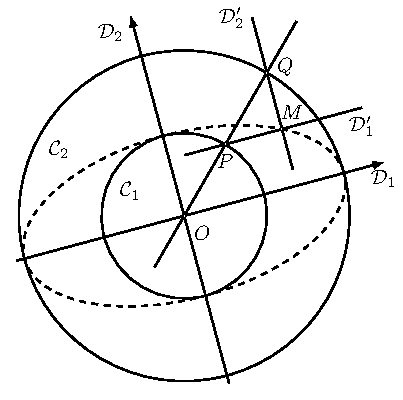
\includegraphics[width=59mm]{img_ellipse_cercles}
    \centering\vspace{-14mm}
  \end{wrapfigure}
  Soient deux droites orthogonales $\ens{D}_{1}$ et $\ens{D}_{2}$ qui se coupent en un point $O$, et deux cercles $\ens{C}_{1}$ et $\ens{C}_{2}$ de centre $O$ et de rayons respectifs $r$ et $R$ avec $0<r<R$.\newline
  Pour tout point $Q$ sur $\ens{C}_{2}$, soit $P=\ens{C}_{1}\cap [O,Q]$.
  Soient $\ens{D}'_{1}$ et $\ens{D}'_{2}$ les deux droites parallèles à $\ens{D}_{1}$ et $\ens{D}_{2}$ et passant par $P$ et $Q$ respectivement.

  On considère le point d'intersection de ces deux droites $M=\ens{D}'_{1}\cap \ens{D}'_{2}$.

  Montrer que quand $Q$ parcourt $\ens{C}_{2}$ le point $M$ parcourt une ellipse.

\end{exo}

\begin{solution}

  On se place dans un repère orthonormé de centre $O$ et d'axes $\ens{D}_{1}$ et $\ens{D}_{2}$. Dans ce repère si $P=(x_{P},y_{P})$ et $Q=(x_{Q},y_{Q})$, alors d'une part $(x_{P},y_{P})=\frac{r}{R}(x_{Q},y_{Q})$, car $P$ est l'image de $Q$ par l'homothétie de centre $O$ et de rapport $\frac{r}{R}$, et d'autre part $M=(x_{Q},y_{P})$ par la construction de $M$, et donc $M=(x_{Q},\frac{r}{R}y_{Q})$.\newline
  Ainsi quand $Q$ parcourt $\ens{C}_{2}$ ayant pour équation $\big\{ x^{2}+y^{2}=R^{2} \big\}$, $M$ parcourt l'image de $\ens{C}_{2}$ par l'affinité $(x,y)\mapsto(x,\frac{r}{R}y)$, qui est l'ellipse dont l'équation dans ce repère orthonormé est\vspace{-.7\baselineskip}
  \[
    \Big(\frac{x}{R}\Big)^{2}+\Big(\frac{y}{r}\Big)^{2}=1.
  \]
  \vspace{-2\baselineskip}

\end{solution}


%-----------------------------------
\begin{exo} (Géométrie dans le plan complexe)

  Cet exercice est relié à la construction d'une approximation de la «spirale d'or» représentée sur la figure.

  \vspace{-2\baselineskip}
  \begin{center}
    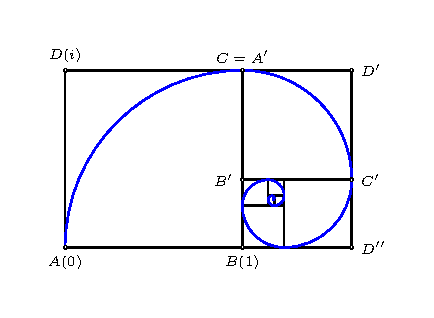
\includegraphics[width=91mm]{img_spirale_or}
  \end{center}
  \vspace{-\baselineskip}

  On se place dans le plan euclidien identifié avec $\mathbb{C}$. Soient $A$, $B$ et $D$ trois points d'affixes respectivement $0$,$1$ et $i$. On considère le carré $ABCD$. On note $\gamma=\frac{1+\sqrt{5}}{2}$ le «nombre d'or».
  Il peut être utile de savoir que $\gamma=1+\frac{1}{\gamma}$.
  \begin{enumerate}
    \item Soient $A'=C$ et $B' \in [BC]$ tel que $\gamma\norm{A'B'}=1$. On considère le carré $A'B'C'D'$ construit à l'extérieur du carré $ABCD$. Montrer qu'il existe une unique transformation affine $S$ qui envoie $ABCD$ sur $A'B'C'D'$ en respectant les sommets ($S(A)=A'$, $S(B)=B'$, \dots).
    \item Soient $z$ l'affixe d'un point $M$ et $S(z)$ l'affixe de son image $S(M)$. Exprimer $S(z)$ en fonction de $z$ et $\gamma$.
    \item Quelle est la nature de $S$ ? Quelle est la nature de $\gamma S$ ?
    \item Déterminer l'ensemble des points fixes de $S$.
    \item Soit $D''=S(D')$. Montrer que $ADD'D''$ est un rectangle. Puis montrer que pour tout $n \in \mathbb{N}$, $S^{\, n}(ABCD) \subset ADD'D''$.
    \item Montrer que $S^{\, 3}(D)=B$.
      Existe-t-il un autre $n \in \mathbb{N}$ pour lequel on a la même relation $S^{\, n}(D)=B$ ?
  \end{enumerate}

\end{exo}

\begin{solution}
  \begin{enumerate}
    \item Soient $T_{\vv{AC}}$ la translation qui envoie $A$ sur $A'=C$, $R_{A,-\frac{\pi}{2}}$ la rotation de centre $A$ et d'angle $-\frac{\pi}{2}$, et $H_{A,\frac{1}{\gamma}}$ l'homothétie de centre $A$ et de rapport $\frac{1}{\gamma}$. Alors $S=T_{\vv{AC}}\circ R_{A,-\frac{\pi}{2}}\circ H_{A,\frac{1}{\gamma}}$ envoie $ABCD$ sur $A'B'C'D'$.\newline
    Par ailleurs cette transformation est unique car il existe une seule transformation qui envoie le repère (orthonormé) $(A,B,D)$ sur le repère (orthogonal) $(A',B',D')$.
    \item L'affixe de $\vv{AC}$ est $1+i$ et donc $T_{\vv{AC}}(z)=z+1+i$. Et comme $H_{A,\frac{1}{\gamma}}(z)=\frac{1}{\gamma}z$ et $R_{A,-\frac{\pi}{2}}(z)=-iz$, on trouve\vspace{-.7\baselineskip}
    \[
      S(z)=-\frac{i}{\gamma}z+1+i.
    \]
    \item L'application $S$ est de la forme $S(z)=az+b$ avec $|a|=\frac{1}{\gamma}$, donc c'est une similitude de rapport $\frac{1}{\gamma}$. Nous avons $\gamma S(z)=-iz+\gamma+i\gamma$ et comme $|-i|=1$ et $-i \neq 1$ c'est une rotation (d'angle $-\frac{\pi}{2}$).
    \item $S(z)=z \ssi -\frac{i}{\gamma}z+1+i=z \ssi z=\gamma \frac{1+i}{\gamma+i}$. Donc $S$ possède un unique point fixe (le centre de la similitude) d'affixe $\gamma \frac{1+i}{\gamma+i}$.
    \item L'affixe de $D'$ est $\gamma+i$ car $S(i)=-\frac{i}{\gamma}i+1+i=\frac{1}{\gamma}+1+i=\gamma+i$ (on utilise que $\frac{1}{\gamma}+1=\gamma$), et celle de $D''$ est $\gamma$ car $S(\gamma+i)=-\frac{i}{\gamma}(\gamma+i)+1+i=\frac{1}{\gamma}+1=\gamma$.\newline
    Comme les affixes de $D$ et $D''$ sont la partie imaginaire et réelle respectivement de l'affixe de $D'$, et l'affixe de $A$ et $0$, alors $ADD'D''$ est un rectangle.\newline
    Vu que $ABCD \subset ADD'D''$, pour montrer que $S^{\, n}(ABCD) \subset ADD'D''$ il suffit de montrer que $S^{\, n}(ADD'D'') \subset ADD'D''$. Et pour démontrer cette dernière inclusion il suffit de montrer que $ADD'D''$ est stable par $S$, c.-à-d. que $S(ADD'D'') \subset ADD'D''$. Mais $S(A)=A'$, $S(D)=D'$, $S(D')=D''$ et $S(D'')=B$ car $S(\gamma)=-\frac{i}{\gamma}\gamma+1+i=1$. Ainsi $S(ADD'D'') = A'D'D''B \subset ADD'D''$.
    \item Nous avons déjà montré dans la question précédente que $S^{3}(D)=S^{2}(D')=S(D'')=B$. Soit $\Omega$ ($\neq B$) le point fixe de $S$, comme $d(\Omega,S^{k}(B))=\big(\frac{1}{\gamma}\big)^{k}d(\Omega,B) \neq d(\Omega,B)$ pour $k \neq 0$ on a $S^{n}(D)=S^{n-3}(B) \neq B$ pour $n-3 \neq 0$.
  \end{enumerate}
\end{solution}

\end{document}
